%%tissue separation
\section{Statistical laws differentiate by tissue}
Observing the GTEx dataset of healthy samples it is possible to study how it is possible to see the tissue differentation and how to study tissues' differences,~\cite{mele2014} suggests the approach.

First of all could be interesting to study which is the fraction of trascriptome that can be explained by a certain number of genes.
One can reduce the realisations to the ones that share the tissue. Than one extimates the average per each component (gene), at this point one has the average abundance of each gene in a tissue, dividing by the sum of all the components it is possible to obtain the fraction of the total counts in the tissue due to each gene. Sorting from greater to smaller and integrating (cumulative summing) one have the fraction of trascriptome due to $1, 2, 3\dots$ genes. This is plot in~\ref{fig:structure/gtex/fraction_of_trascriptome}. 
\begin{figure}[htb!]
  \centering
  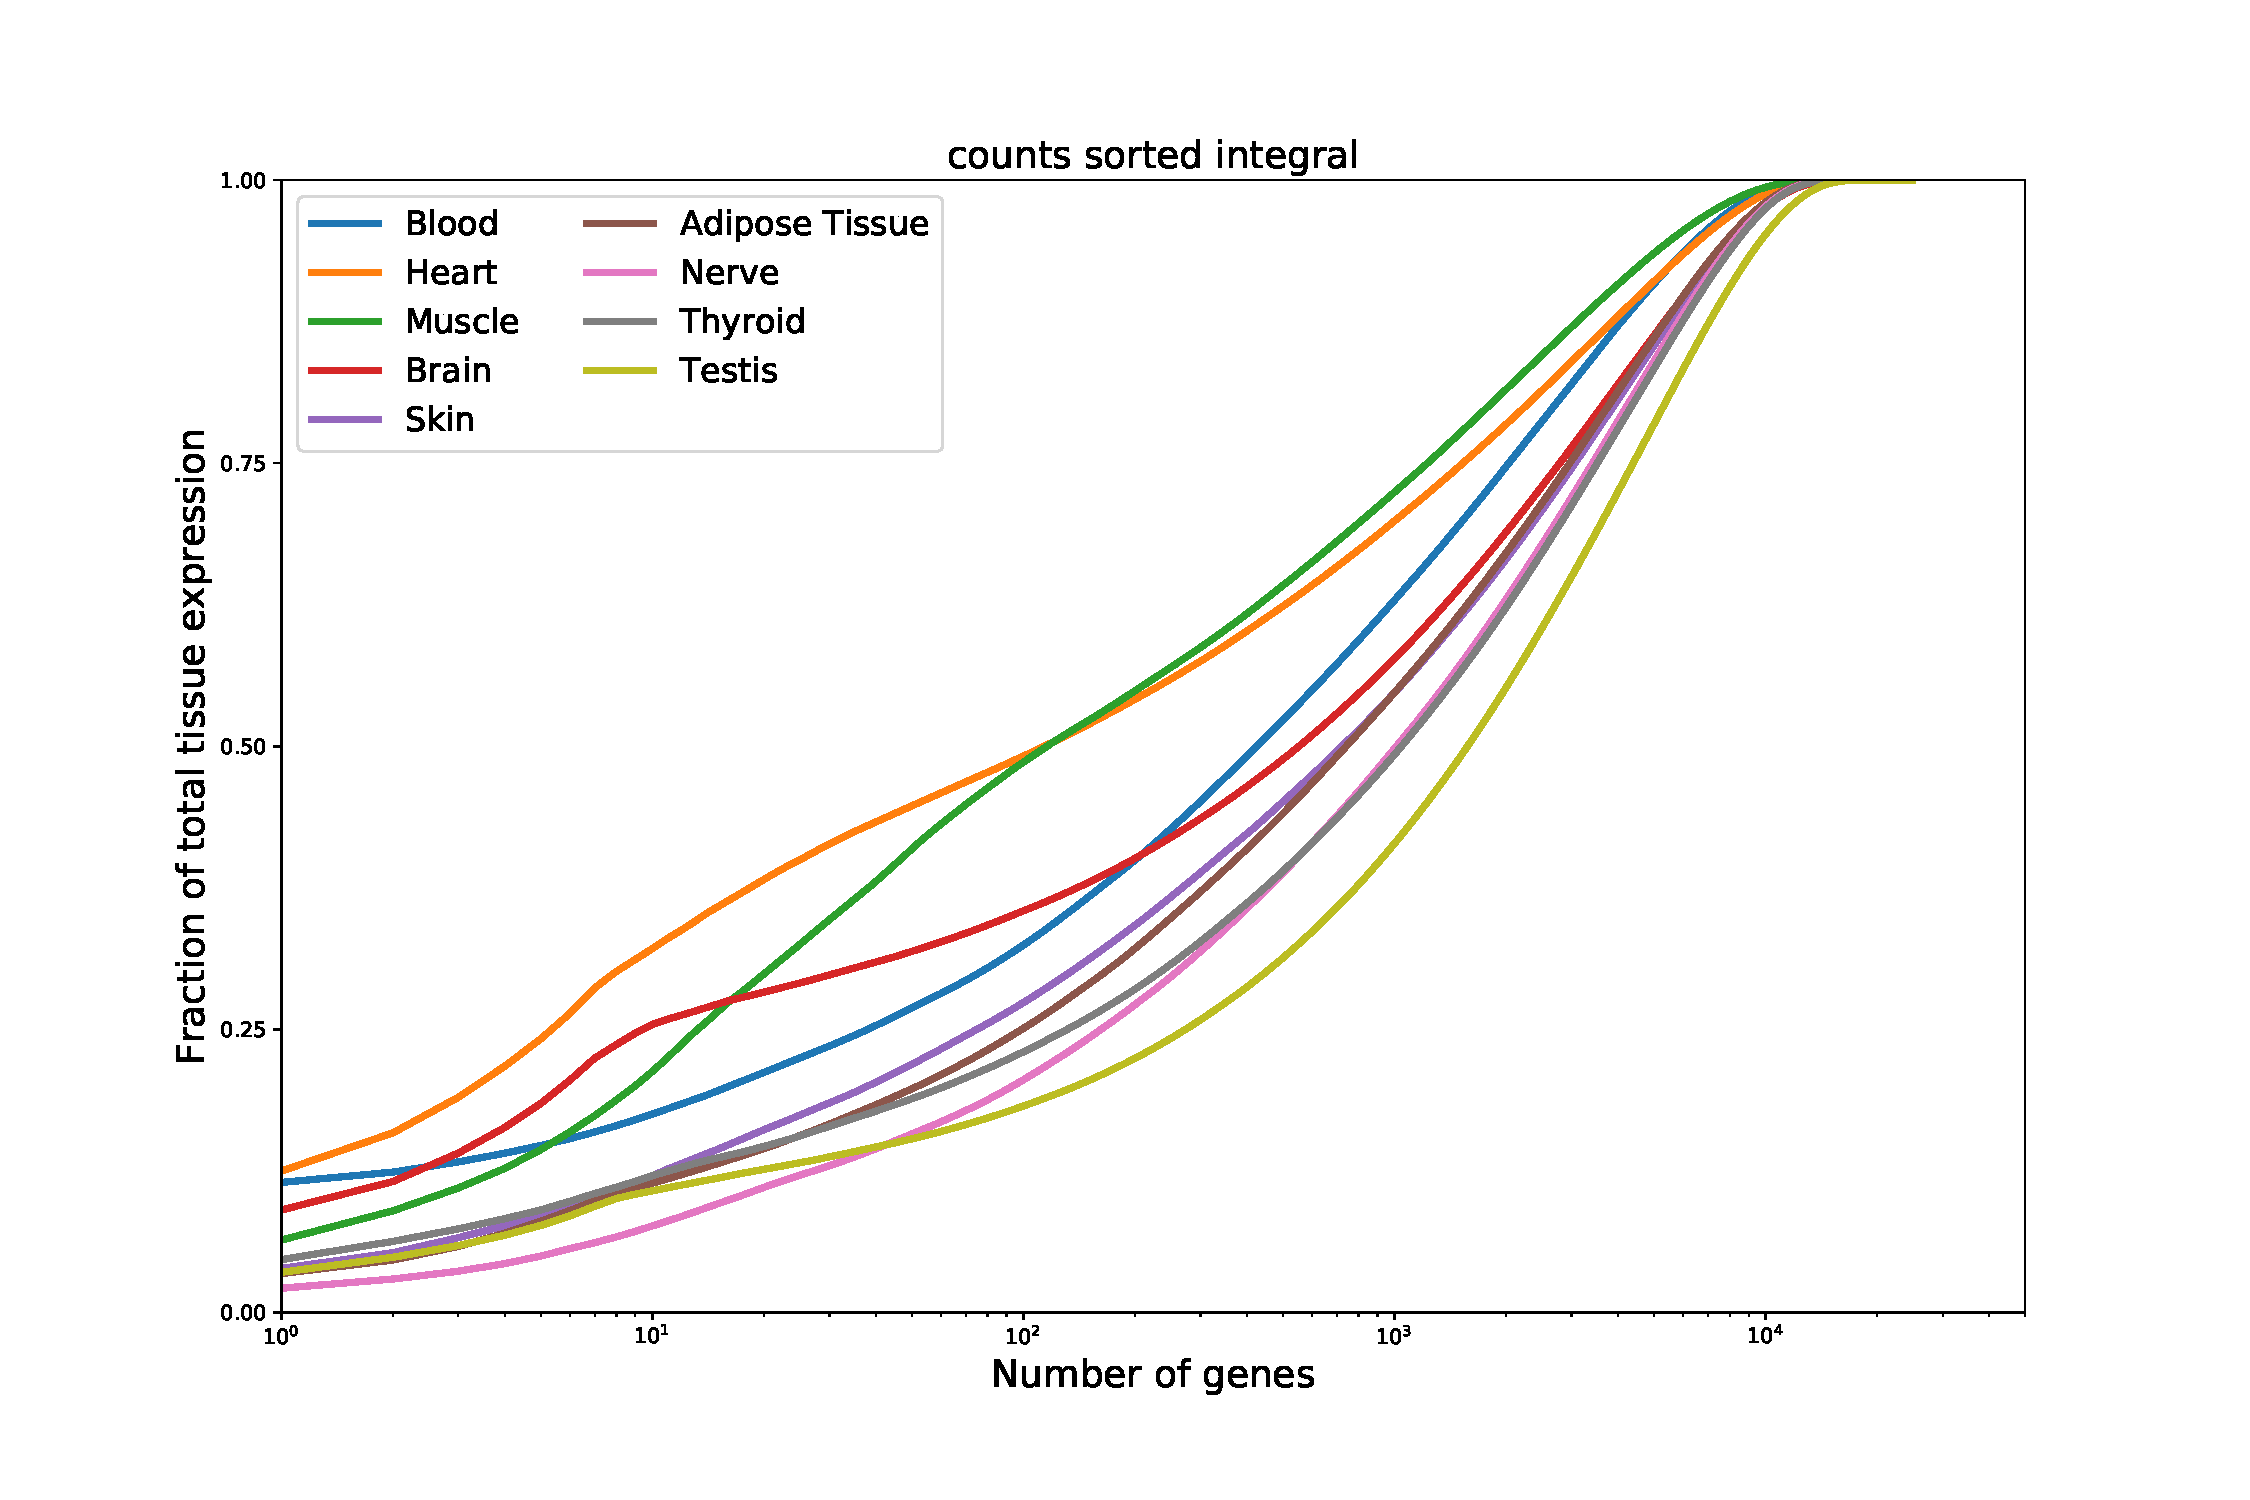
\includegraphics[width=0.9\linewidth]{pictures/structure/gtex/fraction_of_trascriptome.pdf}
  \caption{The integral of the sorted abundances for each tissue}
  \label{fig:structure/gtex/fraction_of_trascriptome}
\end{figure}
Here, if a curve is steep it means that a few genes' counts represent a great fraction of the total. If a curve is smooth it means that many genes are necessary to describe the whole trascriptome for that particular tissue.
This analisys shows that different tissues have a different complexity in terms of the number of genes necessary to build the trascriptome (in average).
In figure~\ref{fig:structure/gtex/fraction_of_trascriptome_Brain} the same analisys is done for the subtissues of Brain, also this subtype separate by tissue.
\begin{figure}[htb!]
  \centering
  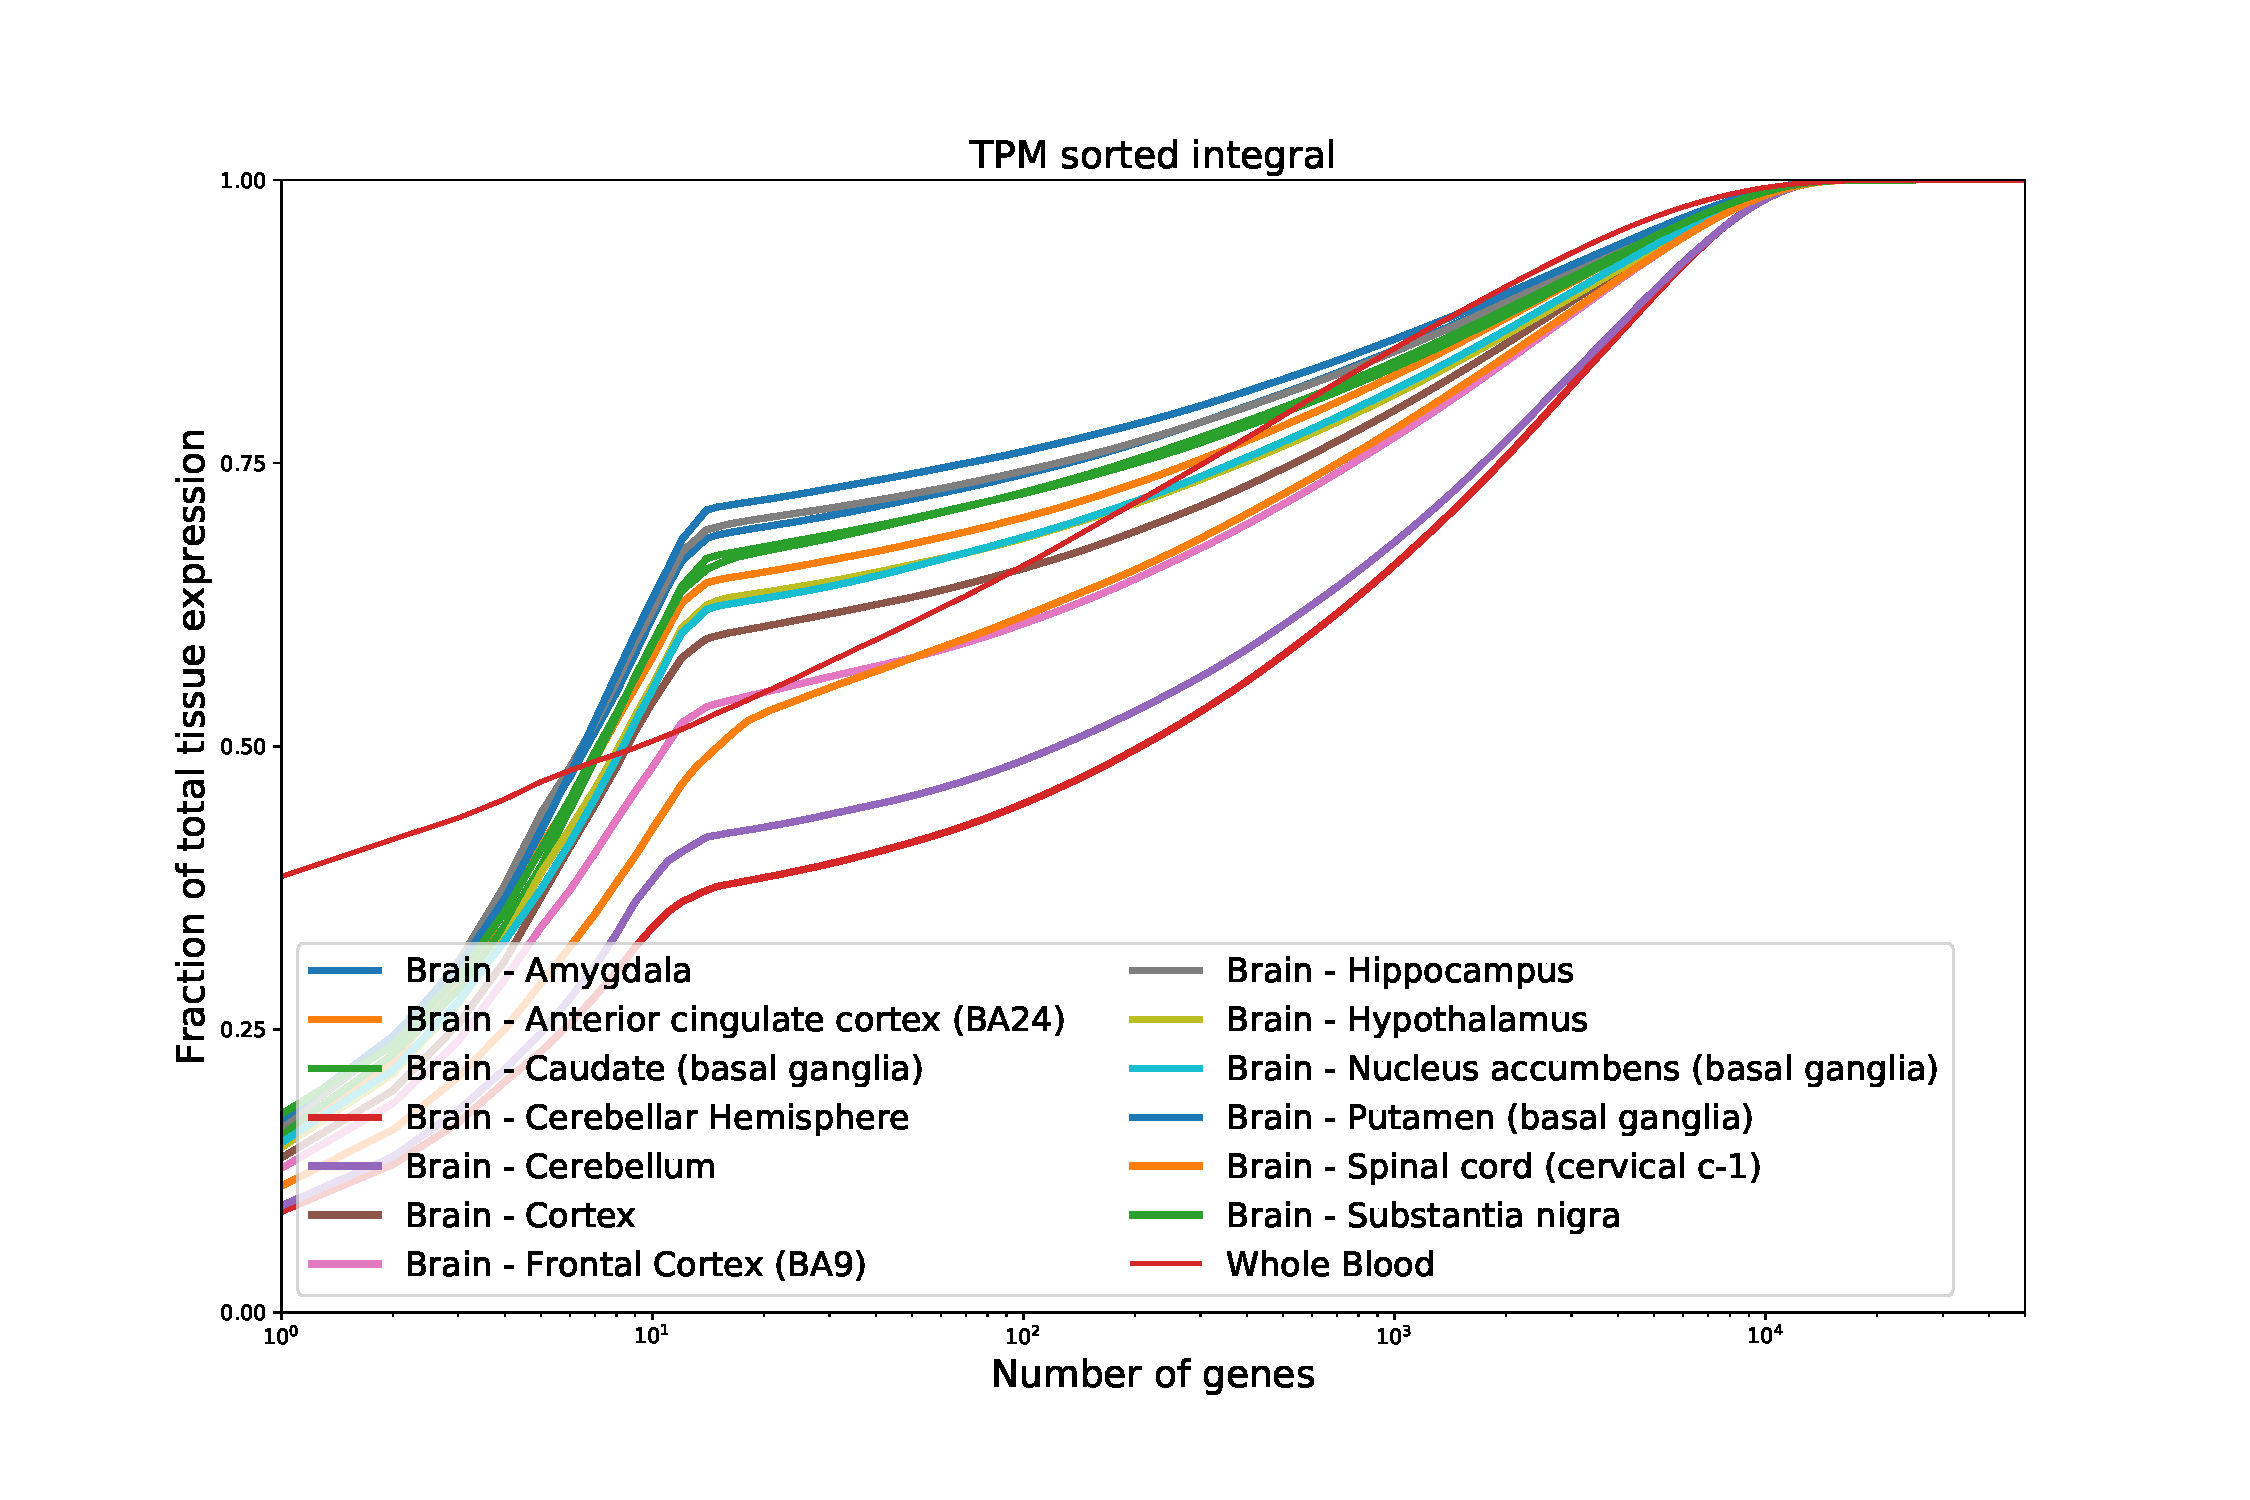
\includegraphics[width=0.9\linewidth]{pictures/structure/gtex/fraction_of_trascriptome_Brain.pdf}
  \caption{The integral of the sorted abundances for subtypes of Brain. This is done using TPM to avoid biases due to gene lenghts. Blood is plotted for reference.}
  \label{fig:structure/gtex/fraction_of_trascriptome_Brain}
\end{figure}

Coming back to the Zipf's law~\ref{eq:zipf}, it is now obvious that~\ref{fig:structure/gtex/fraction_of_trascriptome} represents nothing but the integral of the Zipf's law. So extimating the Zipf looking at a tissue a time, it is evident that each tissue has its particular slope. The steeper the Zipf the simplest is the tissue: the tracriptome can be described with a few genes. In figure~\ref{fig:structure/gtex/zipf_tissue} the tissue with an extremal behaviour.
\begin{figure}[htb!]
  \centering
  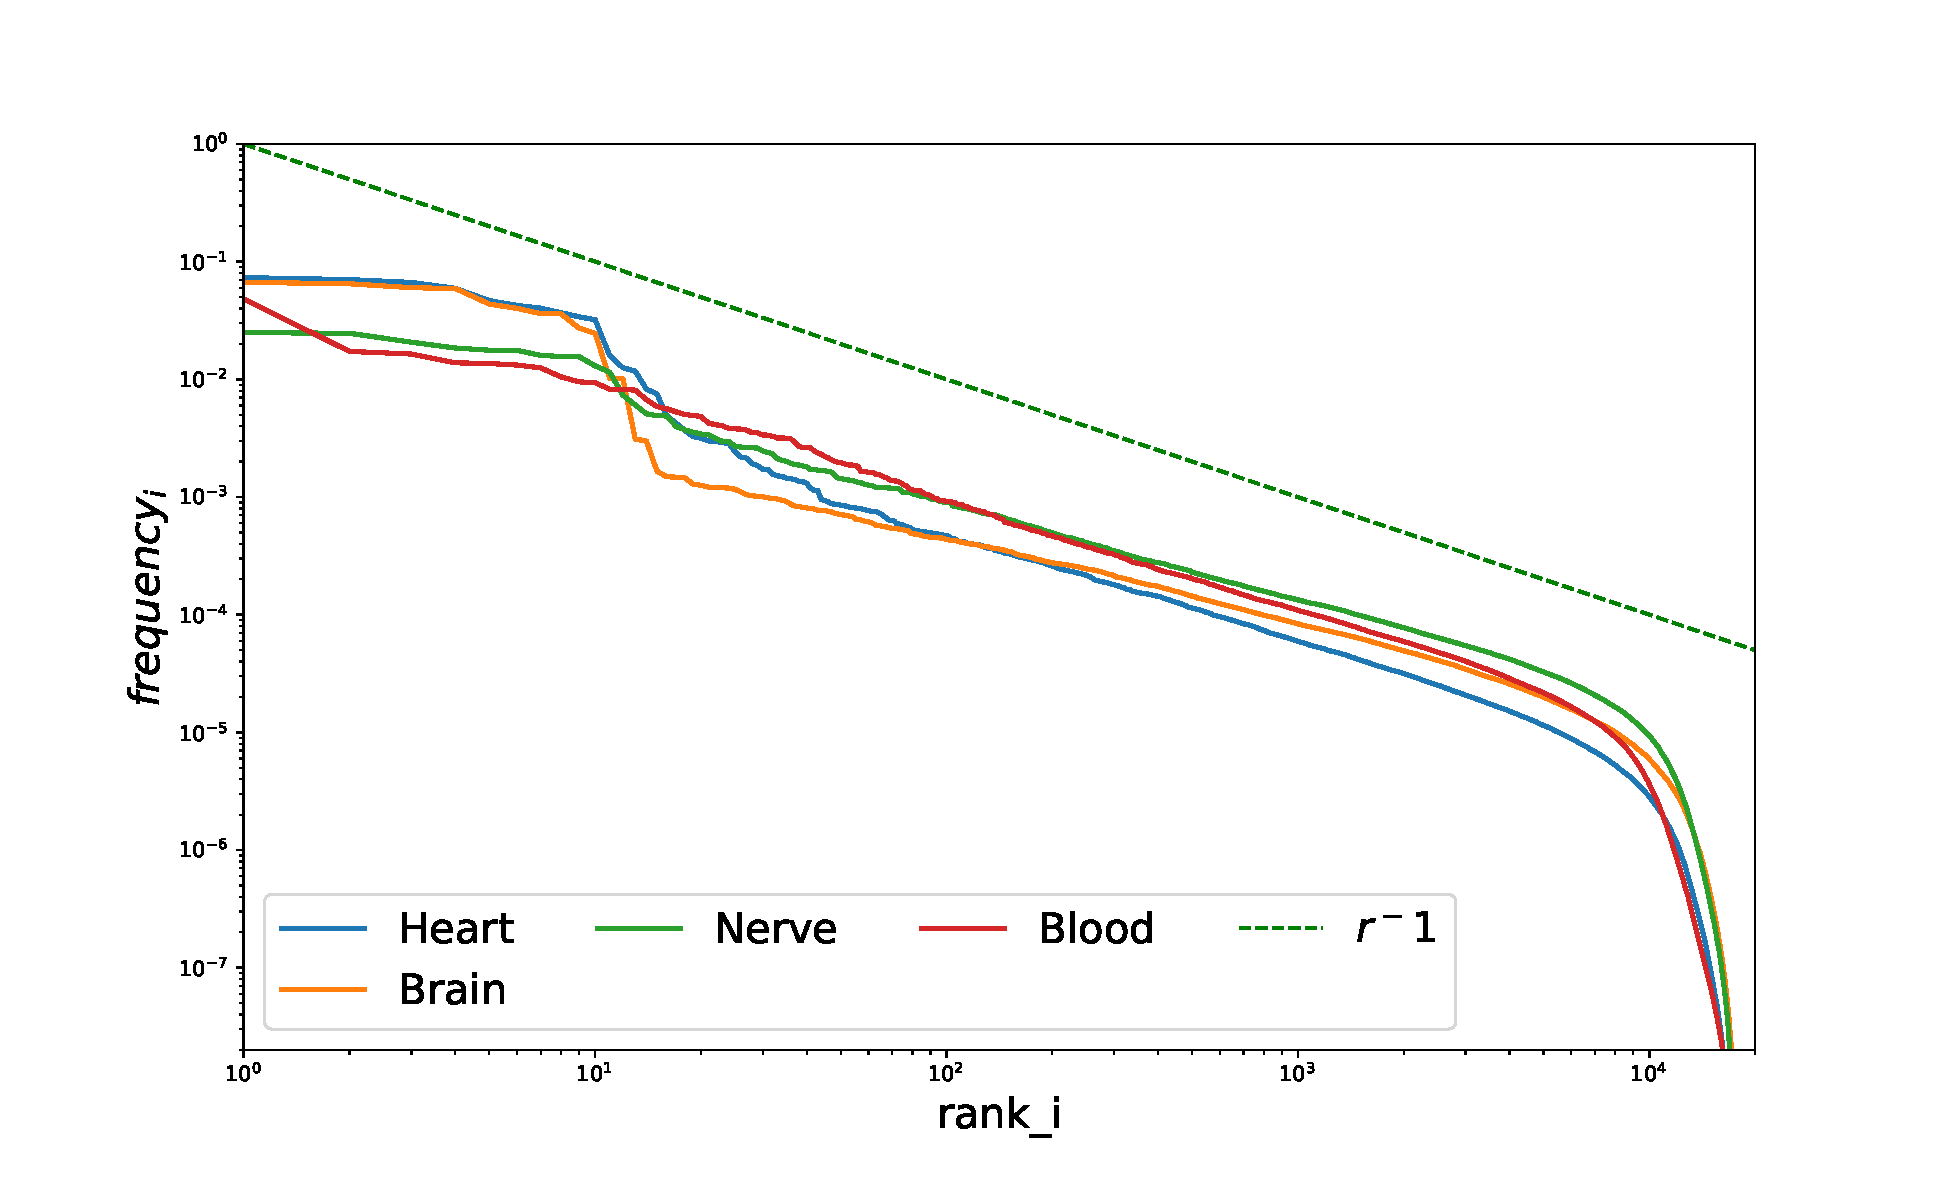
\includegraphics[width=0.6\linewidth]{pictures/structure/gtex/zipf_tissue.pdf}
  \caption{The integral of the sorted abundances for each tissue}
  \label{fig:structure/gtex/zipf_tissue}
\end{figure}

The point where the~\ref{fig:structure/gtex/fraction_of_trascriptome} reaches $1$ corresponds to the total number of genes expressed, the remaining ones have a $0$ expression and do not contribute to the trascriptome. This can be visualized again with the Heaps' law. In figure~\ref{fig:structure/gtex/heaps_tissue} it is evident that there is some kind of tissue differentation even when looking at the Heaps' law.
\begin{figure}[htb!]
  \centering
  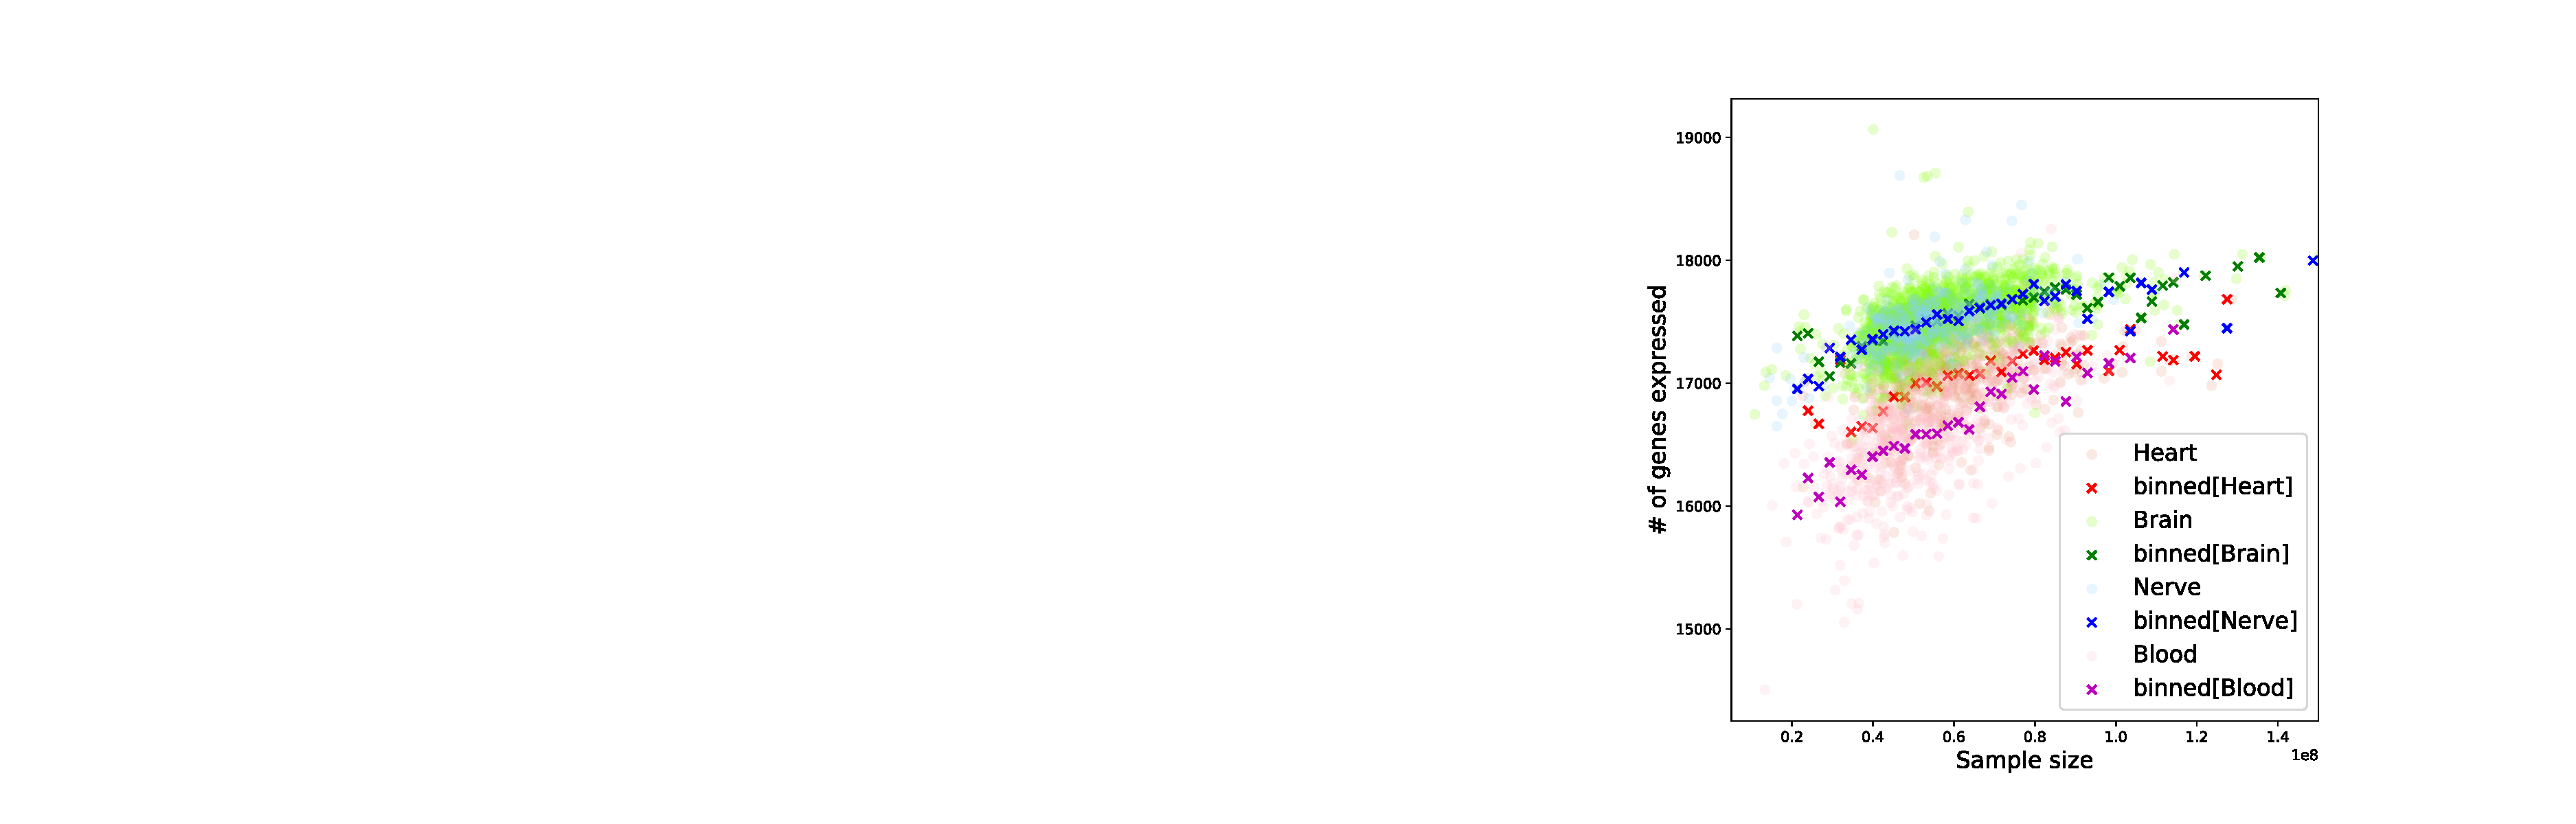
\includegraphics[width=0.6\linewidth]{pictures/structure/gtex/heaps_tissue.pdf}
  \caption{The integral of the sorted abundances for each tissue}
  \label{fig:structure/gtex/heaps_tissue}
\end{figure}

All these analysis suggest that there must be a sort of hidden structure in the data that is somehow related with the tissue each sample comes from. In particular there are many different Zipf's laws hidden behind the data and each sample is build looking at one of these a time. Also given two samples with a similar size, it happens that the number of genes necessary to build that realisation is not always the same (shown by Heaps' law) and it is somehow related to the tissue of the sample.
